\documentclass[english,floatsintext,man]{apa6}

\usepackage{amssymb,amsmath}
\usepackage{ifxetex,ifluatex}
\usepackage{fixltx2e} % provides \textsubscript
\ifnum 0\ifxetex 1\fi\ifluatex 1\fi=0 % if pdftex
  \usepackage[T1]{fontenc}
  \usepackage[utf8]{inputenc}
\else % if luatex or xelatex
  \ifxetex
    \usepackage{mathspec}
    \usepackage{xltxtra,xunicode}
  \else
    \usepackage{fontspec}
  \fi
  \defaultfontfeatures{Mapping=tex-text,Scale=MatchLowercase}
  \newcommand{\euro}{€}
\fi
% use upquote if available, for straight quotes in verbatim environments
\IfFileExists{upquote.sty}{\usepackage{upquote}}{}
% use microtype if available
\IfFileExists{microtype.sty}{\usepackage{microtype}}{}

% Table formatting
\usepackage{longtable, booktabs}
\usepackage{lscape}
% \usepackage[counterclockwise]{rotating}   % Landscape page setup for large tables
\usepackage{multirow}		% Table styling
\usepackage{tabularx}		% Control Column width
\usepackage[flushleft]{threeparttable}	% Allows for three part tables with a specified notes section
\usepackage{threeparttablex}            % Lets threeparttable work with longtable

% Create new environments so endfloat can handle them
% \newenvironment{ltable}
%   {\begin{landscape}\begin{center}\begin{threeparttable}}
%   {\end{threeparttable}\end{center}\end{landscape}}

\newenvironment{lltable}
  {\begin{landscape}\begin{center}\begin{ThreePartTable}}
  {\end{ThreePartTable}\end{center}\end{landscape}}




% The following enables adjusting longtable caption width to table width
% Solution found at http://golatex.de/longtable-mit-caption-so-breit-wie-die-tabelle-t15767.html
\makeatletter
\newcommand\LastLTentrywidth{1em}
\newlength\longtablewidth
\setlength{\longtablewidth}{1in}
\newcommand\getlongtablewidth{%
 \begingroup
  \ifcsname LT@\roman{LT@tables}\endcsname
  \global\longtablewidth=0pt
  \renewcommand\LT@entry[2]{\global\advance\longtablewidth by ##2\relax\gdef\LastLTentrywidth{##2}}%
  \@nameuse{LT@\roman{LT@tables}}%
  \fi
\endgroup}


  \usepackage{graphicx}
  \makeatletter
  \def\maxwidth{\ifdim\Gin@nat@width>\linewidth\linewidth\else\Gin@nat@width\fi}
  \def\maxheight{\ifdim\Gin@nat@height>\textheight\textheight\else\Gin@nat@height\fi}
  \makeatother
  % Scale images if necessary, so that they will not overflow the page
  % margins by default, and it is still possible to overwrite the defaults
  % using explicit options in \includegraphics[width, height, ...]{}
  \setkeys{Gin}{width=\maxwidth,height=\maxheight,keepaspectratio}
\ifxetex
  \usepackage[setpagesize=false, % page size defined by xetex
              unicode=false, % unicode breaks when used with xetex
              xetex]{hyperref}
\else
  \usepackage[unicode=true]{hyperref}
\fi
\hypersetup{breaklinks=true,
            pdfauthor={},
            pdftitle={Race-based disparities in allocation of academic disciplinary actions are associated with county-level rates of bias},
            colorlinks=true,
            citecolor=blue,
            urlcolor=blue,
            linkcolor=black,
            pdfborder={0 0 0}}
\urlstyle{same}  % don't use monospace font for urls

\setlength{\parindent}{0pt}
%\setlength{\parskip}{0pt plus 0pt minus 0pt}

\setlength{\emergencystretch}{3em}  % prevent overfull lines

\ifxetex
  \usepackage{polyglossia}
  \setmainlanguage{}
\else
  \usepackage[english]{babel}
\fi

% Manuscript styling
\captionsetup{font=singlespacing,justification=justified}
\usepackage{csquotes}
\usepackage{upgreek}

 % Line numbering
  \usepackage{lineno}
  \linenumbers


\usepackage{tikz} % Variable definition to generate author note

% fix for \tightlist problem in pandoc 1.14
\providecommand{\tightlist}{%
  \setlength{\itemsep}{0pt}\setlength{\parskip}{0pt}}

% Essential manuscript parts
  \title{Race-based disparities in allocation of academic disciplinary actions
are associated with county-level rates of bias}

  \shorttitle{Discipline Disparities}


  \author{Travis Riddle\textsuperscript{1}~\& Stacey Sinclair\textsuperscript{1}}

  \def\affdep{{"", ""}}%
  \def\affcity{{"", ""}}%

  \affiliation{
    \vspace{0.5cm}
          \textsuperscript{1} Princeton University  }

  \authornote{
    \newcounter{author}
    Enter author note here.

                      Correspondence concerning this article should be addressed to Travis Riddle. E-mail: \href{mailto:triddle@princeton.edu}{\nolinkurl{triddle@princeton.edu}}
                          }


  \abstract{Enter abstract here.}
  \keywords{keywords \\

    \indent Word count: X
  }





\usepackage{amsthm}
\newtheorem{theorem}{Theorem}
\newtheorem{lemma}{Lemma}
\theoremstyle{definition}
\newtheorem{definition}{Definition}
\newtheorem{corollary}{Corollary}
\newtheorem{proposition}{Proposition}
\theoremstyle{definition}
\newtheorem{example}{Example}
\theoremstyle{remark}
\newtheorem*{remark}{Remark}
\begin{document}

\maketitle

\setcounter{secnumdepth}{0}



\section{Introduction}\label{introduction}

\section{Methods}\label{methods}

\subsection{Data Sources}\label{data-sources}

We used three distinct data sources for the work described here. The
academic disciplinary data is part of the Civil Rights Data Collection
(CRDC) through the US Department of Education. The dataset we used comes
from the 2013-2014 academic year and has data on \enquote{all public
local and educational agencies and schools, including long-term secure
juvenile justice facilities, charter schools, alternative schools, and
schools serving students with disabilities.} In total, the CRDC data
represents 95507 institutions enrolling approximately 50 million
students, of which approximately 25 million are white and 7.8 million
are Black\footnote{We note that there are a number of differences
  between the analyses we registered and those presented in the main
  text. Our general conclusions are largely the same for both sets of
  analyses. We opted to report the modified analyses for reasons of
  clarity and to remain congruent with previous research on the same
  topics. The registered analyses can be found, in full, in the
  appendix.}. Previous work using these data have identified a number of
districts whose data are in error, and have excluded juvenile justice
facilities, as these institutions constitute dramatically different
educational environments, where the meaning of disciplinary actions may
be quite different (Losen et al., 2015). After these exclusions are
applied, the final sample used for modeling consists of 90002
institutions, enrolling 32 million black or white students, of which 25
million are white and 7 million are black.

We obtained county-level demographic information for use as covariates
and state-level demographic information for use in post-stratification
from the US Census Bureau. For both county-level and state-level
demographics, we use 5-year estimates for the period ending in 2014 from
the American Community Survey, which surveys around 295k households per
month.

We used measurements of implicit and explicit bias available from data
collected through Project Implicit (Xu, Nosek, \& Greenwald, 2014). From
this data, we used only respondents who had geographic information that
would allow us to place them in a United States county, identified as
White, and visited the site before 2015. This consisted of approximately
1.1 million total respondents from 3091 counties.

A subset of years in the Project Implicit data also collected
occupational information from respondents. As identified in our
pre-analysis plan, we took advantage of the presence of primary and
secondary educators in these data to test whether any associations
between bias and race-based differences in the rates of disciplinary
action were stronger among these respondents. Filtering for only white
individuals who identified as primary, secondary, special education, and
other teachers and instructors (occupation codes 25-2000 and 25-3000)
reduced the dataset to 63552 respondents. In order to assure that our
estimates were reasonably stable, we limited analysis to only counties
that had at least 50 respondents. As such, our teacher analysis is
limited to just 287 counties. Additionally, because we do not know of
any state-level demographic estimates for teachers, we are unable to
perform post-stratification for these data.

\subsection{Measures}\label{measures}

The primary outcome in this analysis is a count of the number of
students by race (black and white) who received one of several types of
disciplinary action. We report here rates of out-of-school suspension,
in-school suspension, school-related arrests, law enforcement referrals,
and total number of expulsions of any type.

For both the post-stratification procedure (described below) and the
actual statistical models used for inference, we used the same set of
covariates. These covariates were at the state-level for
post-stratification and were at the county-level for the statistical
models used for final estimation and inference. Specifically, our
population based covariates were the total population count, the
proportion of the population that is black, the proportion of the
population that is white and the ratio of black-to-white persons. We
also used socioeconomic covariates. We used the percent of individuals
aged 16 or over who were in the labor force but unemployed, the median
household income, and the percentage of all families whose income is
below the poverty line.

Finally, for the implicit and explicit bias measures, we relied on two
primary variables from the Project Implicit data. Implicit bias was
assessed via an Implicit Association Test (IAT). This test uses a
speeded dual-categorization task in which individuals must quickly
categorize black and white faces and \enquote{good} and \enquote{bad}
words with key presses. The difference in how quickly and accurately
participants are able to pair white faces with \enquote{good} words and
black faces with \enquote{bad} words in comparison to the inverse is
thought to reflect implicit associations between the two races and
positive and negative affective reactions. This association is indicated
in the IAT D-score, which we used as a measure of implicit bias. Our
measure of explicit bias is the difference between reported warmth
towards whites (i.e. \emph{how warm or cold do you feel towards Whites?
0=very cold, 10=very warm}) and reported warmth toward blacks.

\subsection{Data analysis}\label{data-analysis}

Data analysis proceded in two steps. We first estimated county-level
implict and explicit bias using multilevel regression and
post-stratification. Post-stratification is a valuable procedure in
obtaining accurate geographical population-based estimates because it
allows a non-representative sample (e.g Project Implicit) to more
closely resemble the true population, and it regularizes extreme
observations with little data to support them (e.g.~a county with only a
handful of respondents with especially high or low scores) (Gelman \&
Little, 1997; Park, Gelman, \& Bafumi, 2004). Following past work
(Leitner, Hehman, Ayduk, \& Mendoza-Denton, 2016), we identified age as
one dimension along which IAT respondents differed from the general
population in ways that could bias our conclusions (Gonsalkorale,
Sherman, \& Klauer, 2009). Our post-stratification weighting scheme is
as follows: We first grouped respondents into five age group categories
(15-24, 25-34, 35-54, 55-75, and 75+). We next fit multilevel models
estimating bias (implicit and explicit biases seperately) as a function
of our state-level covariates (the \enquote{fixed} effects), and allowed
the estimates to vary by age bin, county, and state (the
\enquote{random} effects). Next, we determined the population of whites
in each county in these age groups using the American Community Survey's
5-year estimates ending in 2014. Finally, we used our estimated models
to predict the expected response for each age bin, in each county. Our
final county-level estimates are the average of the values predicted for
the 5 age bins, weighted by the population size of that bin in that
county. As a result of this procedure, we can be confident that our
county-level estimates should more closely approximate what our
estimates would look like if the Project Implicit data were truly
representative along the age dimension in all counties.

After obtaining these estimates, we use them as predictors in bayesian
multilevel logistic regressions. Formally, the likelihood for a given
observation is written as a binomial function:

\[
{n\choose y}\pi^y(1-\pi)^{n-y}
\]

Where \(y\) is the observed count of incidents (e.g.~number of black or
white students suspended), \(n\) is the number of at-risk students
(e.g.~total number of black or white students), and
\(\pi = g^{-1}(\eta)\) is the probability of the incident ocurring. For
this analysis, the linear predictor takes the form of a multilevel model
with a set of effects that vary over county:

\[
\eta = \alpha + X\beta + \gamma_{county}
\]

Where \(\alpha\) is an intercept that is constant across observations,
\(\beta\) represents a set of effects that are also constant across
observations (i.e.~fixed effects), and \(\gamma_{county}\) represents
intercepts and effects of ethnicity that vary across the counties
(i.e.~random efffects).

In addition to the covariates described above, we also include effects
of race, implicit bias, explicit bias, and the two-way interactions
between implicit bias and race and explicit bias and race. We fit
separate models for each of the outcomes.

Because of the computational demands of fitting such a high-dimensional
model to such a large dataset (the full model for each metric would
consist of over 6k parameters to approximately 170k observations), we
used a consensus monte carlo algorithm to obtain approximate posterior
distributions for the parameters of interest (Scott et al., 2016). The
approximate posteriors derived from this algorithm have been shown to be
nearly indistinguishable from the true posterior, a result we verified
using a small subset of our own data.

All numerical predictor variables were standardized at the appropriate
level (county, state) before model estimation to help with estimation
efficiency and interpretability. We set priors for the intercept and
coefficients in the bayesian models to be weakly informative normal
distributions centered on zero with a standard deviation of five. All
other parameters were left to default values. Data analysis was done in
R (R Core Team, 2016) version 3.3.2 running under OS X 10.11.6.
Post-stratification was done with lme4, version 1.1.14 (Bates, Mächler,
Bolker, \& Walker, 2015). Final model fitting was done on the university
cluster running Springdale Linux, release 6.9 using rstanarm, version
2.17.2 (Stan Development Team, 2016). We used the implementation of the
consensus monte carlo algorithm found in parallelMCMCcombine, version
1.0 (Miroshnikov \& Conlon, 2014). Figures were made with ggplot2,
version 2.2.1 (Wickham, 2009), with data manipulation done using dplyr
version 0.7.2 (Wickham, Francois, Henry, \& Müller, 2017) and tidyr,
version 0.7.1 (Wickham \& Henry, 2017). A full report of session
information can be found on the OSF page (\ldots{}.)

\section{Results}\label{results}

\subsection{Project Implicit
Estimates}\label{project-implicit-estimates}

We first report the results of estimating the implicit and explicit
biases in from Project Implicit data. Overall, the individuals in
project implicit show a pro-white bias in both implicit (\emph{mean} =
0.40, \emph{sd} = 0.41), and explicit measures (\emph{mean} = 0.88
\emph{sd} = 1.83). When aggregated at the county level and adjusted with
poststratification, the summary statistics across counties are similar
in terms of their location, but as expected, the variability is much
diminished (\(mean_{implicit}\) = 0.40, \(sd_{implicit}\) = 0.02;
\(mean_{explicit}\) = 0.79, \(sd_{explicit}\) = 0.15, where on both
scales 0 = no bias, and positive numbers indicate a pro-white bias).

\subsection{Disciplinary action
frequency}\label{disciplinary-action-frequency}

\begin{table}[tbp]
\begin{center}
\begin{threeparttable}
\caption{\label{tab:disc-count}Count of students by race receiving each type of disciplinary action}
\begin{tabular}{lll}
\toprule
group & \multicolumn{1}{c}{metric} & \multicolumn{1}{c}{students}\\
\midrule
black & expulsions & 36,755.00\\
black & school arrests & 21,456.00\\
black & in-school suspension & 829,706.00\\
black & law enforcement referral & 53,306.00\\
black & out-of-school suspension & 1,850,492.00\\
white & expulsions & 55,832.00\\
white & school arrests & 21,420.00\\
white & in-school suspension & 1,054,172.00\\
white & law enforcement referral & 81,565.00\\
white & out-of-school suspension & 1,768,326.00\\
\bottomrule
\end{tabular}
\end{threeparttable}
\end{center}
\end{table}

Table \ref{tab:disc-count} shows the number of students of each race who
were reported having received each of the actions under consideration.
The counts range from a low of just 21420 white students arrested to a
high of 1850492 black students receiving an out-of-school suspension.
Considering the vast differences in the overall number of black and
white students, this simple count already illustrates that black
students are disciplined at rates far higher than their white
counterparts.

\subsection{Associations across
county}\label{associations-across-county}

Figure \ref{fig:overall-associations} shows the estimate of primary
interest for each of the models. The estimates displayed are the
coefficients for the interaction between race and each of the two bias
measurements. Given that African Americans are the baseline group,
negative values for this coefficient indicate that as the bias in a
county increases, the gap between the probability of a black student
being disciplined and the probability of a white student being
disciplined grows.

\begin{figure}
\centering
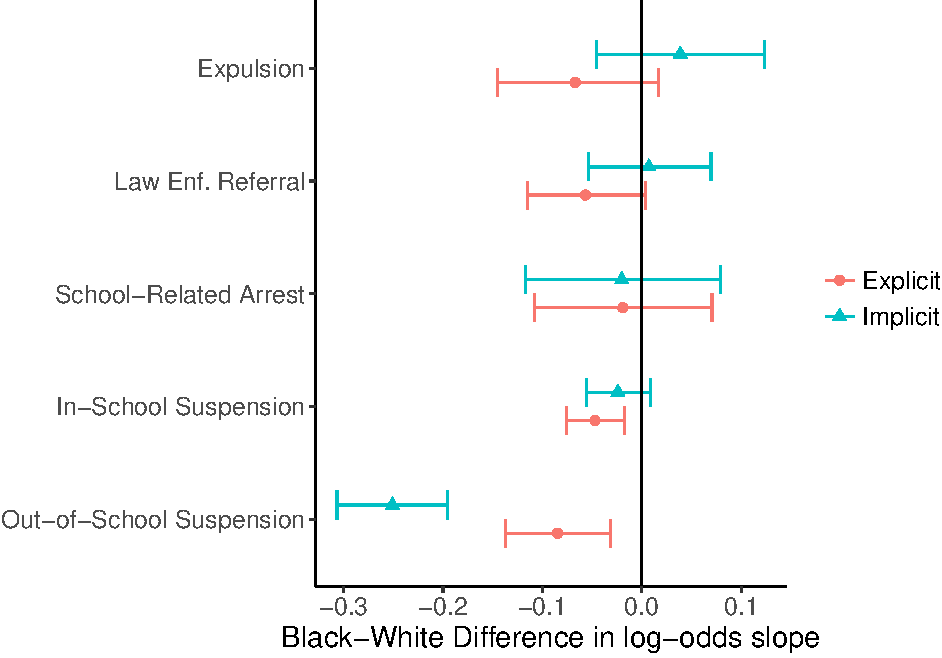
\includegraphics{draft_files/figure-latex/overall-associations-1.pdf}
\caption{\label{fig:overall-associations}Association between each metric and
county-level estimates of explicit and implicit bias. Negative values
indicate that the rate of increase (or decrease) for blacks is faster
(or slower) than for whites. Point is the mean of the posterior and
error bars represent 95\% bayesian uncertainty intervals.}
\end{figure}

Several patterns are apparent from this figure. First, with the
exceptions of implicit bias and expulsions and law enforcement
referrals, all estimates are directionally consistent with higher levels
of bias leading to larger differences between groups. Second, these
effects are especially consistent for the two types of suspensions. The
largest effect estimated is between implicit bias and out-of-school
suspensions. The difference in the slope of the association between
implicit bias and the log of the odds for out-of-school suspensions
between white and black students is estimated to be -0.25, with 95\% of
the posterior distribution between -0.31 and -0.20 and a proportion
\textgreater{}.99 of the posterior distribution consistent with a
negative effect.

Although not nearly as large of a difference, we have similar certainty
with respect to the association between out-of-school suspensions and
explicit bias. The difference in the slope of the association between
explicit bias and the log of the odds for out-of-school suspensions
between white and black students is estimated to be -0.08, with 95\% of
the posterior distribution between -0.14 and -0.03 and a proportion
\textgreater{}.99 of the posterior distribution consistent with a
negative effect.

The estimated associations for in-school suspensions are smaller still,
but are generally consistent with effects of the same direction. For
implicit bias, the relevant parameter is estimated at -0.02 {[}-0.06,
0.01{]} \(p_{neg}\) = 0.93, and for explicit bias, the effect is
slightly larger, and a positive effect is essentially not credible,
given the data and model -0.05 {[}-0.08, -0.02{]} \(p_{neg}\)
\textgreater{}.99.

Other outcomes are estimated with less precision, or with patterns that
are inconsistent between implicit and explicit bias. For instance,
examining the associations for expulsions, the effect of explicit biases
are generally in the expected direction (\emph{est} = -0.07, {[}-0.15,
0.02{]}, \(p_{neg}\) = .94), but the effect for implicit bias is
estimated to be close to zero, with a enough uncertainty (\emph{est} =
0.04, {[}-0.05, 0.12{]}, \(p_{neg}\) = .19) to make it difficult to
claim an effect of one direction or the other. The model indicates
similar uncertainty with respect to school-related arrests and both
estimates of bias (\(est_{explicit}\) = -0.02, {[}-0.11, 0.07{]},
\(p_{neg}\) = .67; \(est_{implicit}\) = -0.02, {[}-0.12, 0.08{]},
\(p_{neg}\) = .66).

\begin{figure}
\centering
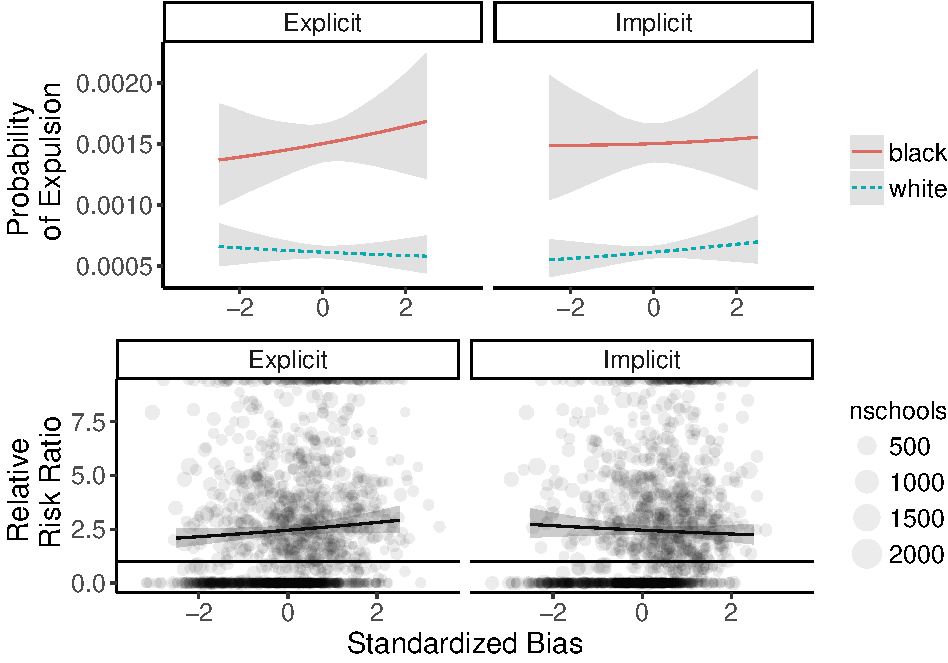
\includegraphics{draft_files/figure-latex/detail-fig-exp-1.pdf}
\caption{\label{fig:detail-fig-exp}Association between bias and expulsions.
Top: Association between bias and the estimated probability of
expulsion. Line is the mean of the posterior. Bands indicate 95\%
uncertainty intervals; Bottom: Association between bias and the relative
risk ratio for black students to white students. Points represent
counties, whose size are scaled to the number of schools in that
county.}
\end{figure}

To better illustrate the nature of these relationships, figure
\ref{fig:detail-fig-exp} shows the estimated probabilities of expulsion
for black and white students as a function of bias, along with the
relative risk ratio for black students. The relative risk ratio is the
ratio of the probability that a black student will be expelled to the
probability that a white student will get expelled. Values over 1
reflect higher levels of punishment for black students. As previously
indicated in table \ref{tab:disc-count}, the top part of this figure
makes plain the higher probability of expulsion for black children. In a
county at the mean of the distribution of bias, approximately 0.15\% of
black students are expected to be expelled {[}0.14, 0.17{]}. The
corresponding rate for white students is much lower, with about 0.06\%
expected to be expelled {[}0.06, 0.07{]}. Moving to a county one
standard deviation above the mean of explicit bias has the effect of
increasing the estimated percentage of black students expected to be
expelled to 0.16\% {[}0.13, 0.18{]}, while the percentage of white
students expected to be expelled would decline to 0.06\% {[}0.05,
0.07{]}. The same movement for implicit bias would slightly increase the
expected expulsions for black students ( 0.15\% {[}0.13, 0.18), and
increase the expected expulsions for white students a very small amount
more to (0.06\% {[}0.06, 0.07). In real terms, in a county at the mean
of the distributions of bias, for every white student expelled, we
should expect 2.45 {[}2.25, 2.45{]} black students to be expelled. If we
move to a county one standard deviation above the mean of explicit bias,
the ratio of black to white students expelled increases to 2.63 {[}2.33,
2.63{]}, while the same movement for implicit bias slightly decreases
the ratio to 2.36 {[}2.13, 2.36{]}.

\begin{figure}
\centering
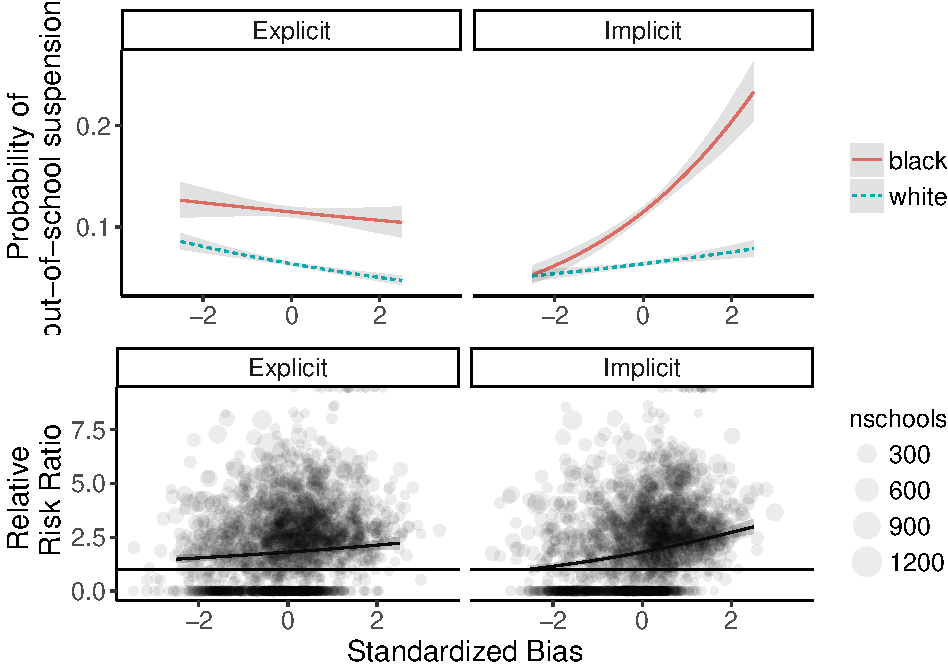
\includegraphics{draft_files/figure-latex/detail-fig-susp-1.pdf}
\caption{\label{fig:detail-fig-susp}Association between bias and
out-of-school suspensions Top: Association between bias and the
estimated probability of suspension Line is the mean of the posterior.
Bands indicate 95\% uncertainty intervals; Bottom: Association between
bias and the relative risk ratio for black students to white students.
Points represent counties, whose size are scaled to the number of
schools in that county.}
\end{figure}

Figure \ref{fig:detail-fig-susp} shows similar patterns, but for
out-of-school suspensions. In a county at the mean of the distribution
of bias, approximately 11.50\% of black students are expected to be
suspended {[}11, 12{]}. The corresponding rate for white students is
just over half that for black students, with about 6.40\% expected to be
suspended {[}6.20, 6.50{]}. Moving to a county one standard deviation
above the mean of explicit bias has the effect of slightly decreasing
the estimated percentage of black students expected to be suspended to
11.10\% {[}10.30, 11.80{]}, while the percentage of white students
expected to be suspended would decrease at a faster rate to 5.60\%
{[}5.40, 5.90{]}. The same movement for implicit bias would dramatically
increase the expected suspensions for black students (15.40\% {[}14.40,
16.40), and increase the expected suspensions for white students a much
smaller amount to (6.90\% {[}6.60, 7.30). In real terms, in a county at
the mean of the distributions of bias, for every white student expelled,
we should expect 1.80 {[}1.73, 1.80{]} black students to be expelled. If
we move to a county one standard deviation above the mean of explicit
bias, the ratio of black to white students expelled increases to 1.96
{[}1.84, 1.96{]}, while the same movement for implicit bias slightly
decreases the ratio to 2.23 {[}2.11, 2.23{]}.`

\section{Discussion}\label{discussion}

\newpage

\section{References}\label{references}

\newpage

\section{Appendix}\label{appendix}

\subsection{Preregistered analysis}\label{preregistered-analysis}

In our preanalysis plan, we specified our analyses to focus on 13
actions - corporal punishment, in-school suspension, out-of-school
suspension, expulsion with educational services, expulsion without
educational services, expulsion under zero-tolerance policies, referral
to law enforcement, school-related arrests, mechanical restraint,
physical restraint, seclusion, preschool suspension, and preschool
expulsion. However, upon further study, we discovered reasons we thought
justified excluding a number of these outcomes. In particular,
seclusion, physical restraint, and mechanical restraint are not
disciplinary actions, but are rather used as means to restrain students
who are at risk of harming themselves or others. Additionally, the
number of preschool students who are expelled or suspended is
vanishingly small (131 total expulsions and 6751 total suspensions out
of over 1.4 million enrolled preschool students), making reliably
estimating any association across counties exceedingly unlikely. We
additionally discovered that counts of one expulsion category (expulsion
under zero-tolerance policies) overlapped with counts in other
categories, and so excluded this category. To remain consistent with
previous studies, we opted to combine the remaining two expulsion
categories to yield one overall count of the number of students
expelled.

We also preregistered our explicit bias as a simple feeling thermometer
towards balcks (i.e. \emph{how warm or cold do you feel towards Blacks?
0=very cold, 10=very warm}). However, past research (Hehman, Flake, \&
Calanchini, 2017; Leitner et al., 2016) has used the difference in
reported warmth towards whites and blacks, and so in the main text, we
report models using this metric of explicit bias. Additionally, we
preregistered analyses with poststratified estimates (as presented in
the main text) along with raw, county-based means. Finally, we had not
known about the issues with juvenile justice facilities, or with the
school districts with reporting errors. Here, we present the results of
the preregistered analyses exactly.

\section{Simple county means}\label{simple-county-means}

\section{Post stratified estimates}\label{post-stratified-estimates}

\section{Teacher analyses}\label{teacher-analyses}

\setlength{\parindent}{-0.5in} \setlength{\leftskip}{0.5in}

\hypertarget{refs}{}
\hypertarget{ref-bates2015fitting}{}
Bates, D., Mächler, M., Bolker, B., \& Walker, S. (2015). Fitting linear
mixed-effects models using lme4. \emph{Journal of Statistical Software},
\emph{67}(1), 1--48.
doi:\href{https://doi.org/10.18637/jss.v067.i01}{10.18637/jss.v067.i01}

\hypertarget{ref-gelman1997poststratification}{}
Gelman, A., \& Little, T. C. (1997). Poststratification into many
categories using hierarchical logistic regression. \emph{Survey
Methodology}, \emph{23}(2), 127--35.

\hypertarget{ref-gonsalkorale2009aging}{}
Gonsalkorale, K., Sherman, J. W., \& Klauer, K. C. (2009). Aging and
prejudice: Diminished regulation of automatic race bias among older
adults. \emph{Journal of Experimental Social Psychology}, \emph{45}(2),
410--414.

\hypertarget{ref-hehman2017disproportionate}{}
Hehman, E., Flake, J. K., \& Calanchini, J. (2017). Disproportionate use
of lethal force in policing is associated with regional racial biases of
residents. \emph{Social Psychological and Personality Science},
1948550617711229.

\hypertarget{ref-leitner2016blacks}{}
Leitner, J. B., Hehman, E., Ayduk, O., \& Mendoza-Denton, R. (2016).
Blacks' death rate due to circulatory diseases is positively related to
whites' explicit racial bias: A nationwide investigation using project
implicit. \emph{Psychological Science}, \emph{27}(10), 1299--1311.

\hypertarget{ref-losen2015we}{}
Losen, D. J., Hodson, C. L., Keith, I., Michael, A., Morrison, K., \&
Belway, S. (2015). Are we closing the school discipline gap?

\hypertarget{ref-miroshnikov2014parallel}{}
Miroshnikov, A., \& Conlon, E. (2014). \emph{ParallelMCMCcombine:
Methods for combining independent subset markov chain monte carlo (mcmc)
posterior samples to estimate a posterior density given the full data
set}. Retrieved from
\url{https://CRAN.R-project.org/package=parallelMCMCcombine}

\hypertarget{ref-park2004bayesian}{}
Park, D. K., Gelman, A., \& Bafumi, J. (2004). Bayesian multilevel
estimation with poststratification: State-level estimates from national
polls. \emph{Political Analysis}, \emph{12}(4), 375--385.

\hypertarget{ref-rcitation}{}
R Core Team. (2016). \emph{R: A language and environment for statistical
computing}. Vienna, Austria: R Foundation for Statistical Computing.
Retrieved from \url{https://www.R-project.org/}

\hypertarget{ref-scott2016bayes}{}
Scott, S. L., Blocker, A. W., Bonassi, F. V., Chipman, H. A., George, E.
I., \& McCulloch, R. E. (2016). Bayes and big data: The consensus monte
carlo algorithm. \emph{International Journal of Management Science and
Engineering Management}, \emph{11}(2), 78--88.

\hypertarget{ref-rstanarm2016}{}
Stan Development Team. (2016). Rstanarm: Bayesian applied regression
modeling via Stan. Retrieved from \url{http://mc-stan.org/}

\hypertarget{ref-wickham2009ggplot2}{}
Wickham, H. (2009). \emph{Ggplot2: Elegant graphics for data analysis}.
Springer-Verlag New York. Retrieved from \url{http://ggplot2.org}

\hypertarget{ref-wickham2017tidyr}{}
Wickham, H., \& Henry, L. (2017). \emph{Tidyr: Easily tidy data with
'spread()' and 'gather()' functions}. Retrieved from
\url{https://CRAN.R-project.org/package=tidyr}

\hypertarget{ref-wickham2017dplyr}{}
Wickham, H., Francois, R., Henry, L., \& Müller, K. (2017). \emph{Dplyr:
A grammar of data manipulation}. Retrieved from
\url{https://CRAN.R-project.org/package=dplyr}

\hypertarget{ref-xu2014psychology}{}
Xu, K., Nosek, B., \& Greenwald, A. (2014). Psychology data from the
race implicit association test on the project implicit demo website.
\emph{Journal of Open Psychology Data}, \emph{2}(1).






\end{document}
